\section{Simulation}

Simulation:
In our project our aim is to implement the feature of voice streaming in the already developed application of Two Tall Totems called Think together. In order to implement this feature we have first developed a model architecture of our design where we’ll be using multiple nodes as the leaf nodes in a network. Then we also have some nodes that act as relayers in the network that will transfer the voice stream from the presenter ( super node) in the network to the corresponding leaf nodes in the network. Along with all these nodes we also have a cloud server which will act as a primary storage device for all the voice streams that will transmitted throughout the network. All the nodes will have a direct link to the server so that if any of the leaf nodes (student nodes) wants to retrieve any voice stream they can do so by making a request to the cloud server for that voice stream directly through the relayer (big node). 





Now after designing the model architecture , we plan to create a working network by creating a simulation using omnet++ a simulation tool. By creating this simulation we’ll have an idea of how the voice stream packets are being transferred between the different nodes present in the network. Once the simulation starts working for a basic scenario of just 2 leaf nodes, a relayer \& a cloud server, we’ll add more number of nodes to the simulation and then analyse what changes are to be made to certain parameters of the network so as to avoid any kind of latency and disturbance while transferring the voice streams. 
As a part of future work, we aim to extend this application for people who can download the voice stream from the presentation remotely in real-time. We also aim to use a hierarchical structure for the network which will help the different nodes present in the network to change their roles during the presentation at any time. Once the application is working perfectly for a limited number of users we aim to extend this application in a way so that it can be used for any number of users without having any storage issues, any disruption in the voice streaming or any bandwidth issues in the network by adding large number of users to the presentation. Another thing that we will take care of in the future is that if any of the relayer nodes fails then all the leaf nodes linked to that relayer will be dynamically transferred to another relayer.


Simple case simulation:

Overview:

The simulation is to test the efficiency in transferring voice data packets with 
a fundamental model. This model lays the groundwork for future expansion. It 
illustrates the simplest way to form a class. The purpose of simulation is to 
investigate the feasibility, and more importantly, the efficiency of the model. 
In the simulation, parameters such as packet drops, delay time etc. are 
collected and extracted to generate an .vec file. The .vec file is then used as 
a foundation for performance analysis.  

To simplify, we assume all the attendees are physically located in the same 
classroom. This will eliminate potential influence caused by the difference of 
location, such as propagation delay. There are five components in the model: 
presenter, relayer, cloud, server and attendee. Each component coordinates with 
one another in order to offer recording services to attendees. There are two 
test cases, one as a small-scaled network with two attendees, the other as 
large-scaled network with ten attendees. The simulation is run in HTTP net, 
masking the lower level network layers such as TCP and IP. 

One can think of the model as a lecture in real life. A presenter is an 
instructor who gives speech up at the front; attendees are students who receive 
the lecture. The voice packets travel via links is the knowledge the instructor 
delivers. The layers and cloud are possible approaches the instructor adopts to 
pass on that knowledge. How well a student understand is not a good predictor of 
instructor’s capability; it largely depends on the media, that is, how well the 
instructor could transfer his thinking in a explanatory way. And that is where 
the cloud and relayers come into play. They are different routes a voice packet 
can travel through. Often attendees receive voice packets through relayers while 
cloud and server provide back-up services. Once the relayers go down, attendees 
will request voice stream from cloud. The cloud 
will take over and serve as the main approach to deliver packets.  Noted that 
only in simple cases where all attendees share the same role do relayers act as 
routers. For more complex scenario, where there are multiple roles for 
attendees, relayers act as filter and only forward packets to the designated 
attendees. 

Model Taxonomy

Below is a overall picture of the simulation model in small-scaled case. It 
breaks down to four  parts: sender(presenter), receiver(attendees), 
mediator(relayers), and backup(cloud and server). 

\begin{figure}[h!]  
  \centering
    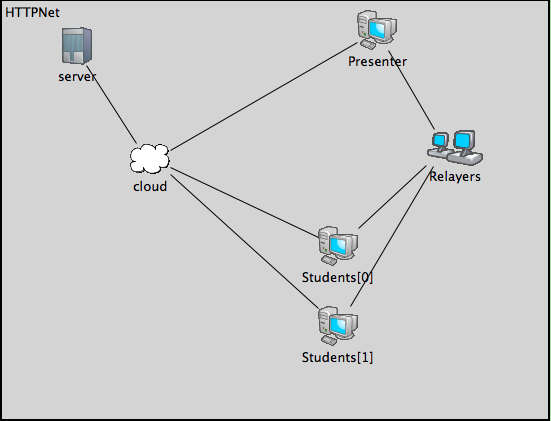
\includegraphics[width=0.5\textwidth]{figures/sce.png}
  \caption{A picture of a gull.}
\end{figure}

Presenter is the starting point of service. It does not rely on any outer 
resource to trigger sending process. Currently no packets other than 
acknowledgement are sent to presenters. In other word, one can view presenters 
as a resource provider and there is no prerequisite for presenters to function. 
There are two outgoing link connected to presenters. The one connected to 
relayers is the main channel for delivering data. The one connected to cloud 
transfer the same content, yet it is less demanding in terms of propagation 
speed and processing time. Presenter send voice packets to both links 
simultaneously, and sets a timer for next cycle. 

Server and Cloud can be considered as a group in terms of services purpose. They 
are both built to provide backup for attendees. There are two scenarios in which 
attendees would need backup services. On one hand, packets are lost by the 
relayers and attendees will ask for complementary data from Cloud to make sure 
smooth stream. On the other hand, sometimes attendees are not able to attend the 
class, but request a later review of that class. It is server that stores the 
lectures in the format of voice stream and deliver it to attendees via Cloud. In 
this regard, Cloud is an interface between service providers and receivers. In 
addition, once network is scaled up to include multiple server, Cloud acts as 
coordinator that organizes servers’ actions. 

Relayer acts as a router in simple case simulation. Unlike servers, relayer does 
not store voice data, thereforegull attendees can not request data from relayer 
later on. Be noted that primary function is not yet implemented, and will be 
addressed later in future model. 

Attendees are students in the diagram. They receive voice packets from 
presenters, regularly through relayers. Be noted that attendees will not send 
acknowledgement back to presenters. When the network between relayers and 
attendees are down, or for some reason, packets are lost in the regular 
transmission routes, attendees will request the data from server. The target 
users of Thinktogether app is attendees and presenters.  
Execution Sequence:

To collect data from multiple cycles, we set a timer for both presenter and 
attendees based on exponential function. After sending the voice packets, 
presenter will create a timer that controls how long before the next cycle, 
namely, the next time it starts sending the packets. The duration of the timer 
is based on a exponential function, which allows random distribution in sending 
packets. The same principle applies to rate of sending request from attendees. 
There is also a timer created by attendee that controls the rate of sending 
requests to cloud. In real life, attendee need complementary data from cloud 
only when relayers fail to deliver it. However, in order to fully evaluate the 
function, in the simulation we config attendee to request voice data from cloud 
whether the relayers go down or not.

\begin{figure}[h!]
  \centering
    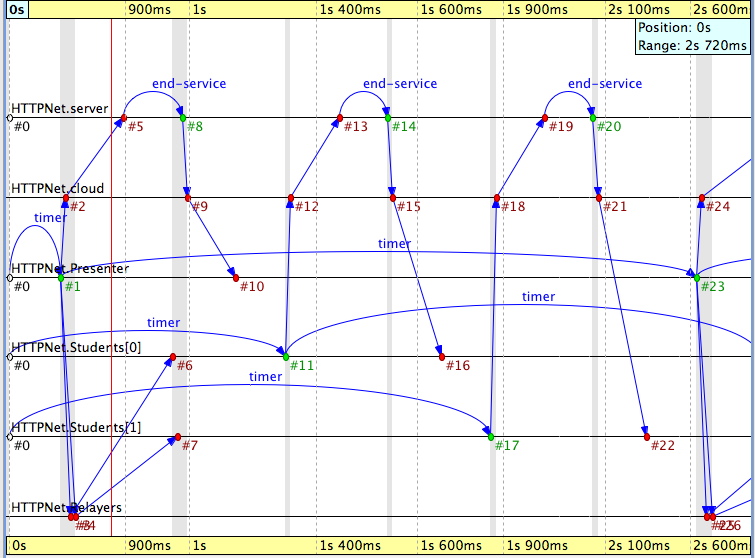
\includegraphics[width=0.5\textwidth]{figures/r_seq.png}
  \caption{A picture of a gull.}
\end{figure}

The execution sequence is illustrated by diagram below. It is a log file 
generated by running a small-scaled cases. 

Presenters initialize services by sending voice packets to both relayers and 
cloud. Then it creates a timer. Upon receiving the packets, server store them 
locally and echoes back an acknowledgement. The services between presenter and 
server is now finished. In other side,
voice packets reach the relayer and will be directed to all attendees relayer 
connects to, which is illustrated by \#6 and \#7 event in diagram. Out of 
testing purpose, each attendees request the exact same voice data from cloud. 
Cloud handles that request by fetching corresponding data in server and sending 
back the requested content. One can refer to events from \#11 to \#16 for 
execution sequence details. 
 


